

%%%%%%%%%%%%%%%%%%%%% LateX template %%%%%%%%%%%%%%%%%


%%%%%%%%%%%% inicio del documento incluyendo opciones %%%%%%%%%%%%%%%%%%%%%%%%%%%%%%%
\documentclass[letterpaper,11pt]{article}
%%%%%%%%%%%%%%%%%%%%%%%%%%%%%%%%%%%%%%%%%%%%%%%%%%%%%%%%%%%%%%%%%%%%%%%%%%%%

%%%%%%% paquetes utiles: español, incluir graficos, etc %%%%%%%%%%%%%%%%%%%%%%%%%%%%
\usepackage[utf8]{inputenc}
\usepackage{amsmath}
\usepackage{amsfonts}
\usepackage{amssymb}
\usepackage{amsthm}
\usepackage[spanish]{babel}
\usepackage{latexsym}
\usepackage{euscript}
\usepackage{graphicx}
\usepackage{tdclock}
\usepackage{braket}
\usepackage[autostyle=true]{csquotes}
\usepackage{braket}
\usepackage{pdfpages}
\usepackage{subcaption}
\usepackage{hyperref}
%%%%%%%%%%%%%%%%%%%%%%%%%%%%%%%%%%%%%%%%%%%%%%%%%%%%%%%%%%%%%%%%%%%%%%%%%%%%%%%%%%

%%%%%%%%%%%%%%%%%%% espacio para la primera linea del parrafo %%%%%%%%%%%%%%%
\setlength{\parindent}{0mm} 
%%%%%%%%%%%%%%%%%%%%%%%%%%%%%%%%%%%%%%%%%%%%%%%%%%%%%%%%%%%%%%%%%%%%%%%%%%

%%%%%%%%%%%%%%% espacio entre parrafos %%%%%%%%%%%%%%%%%%%%%%%%%%%%%%%
\setlength{\parskip}{2mm}
%%%%%%%%%%%%%%%%%%%%%%%%%%%%%%%%%%%%%%%%%%%%%%%%%%%%%%%%%%%%%%%%%%%%

%%%%%%%%%%%%%%%%%%%%% espaciado entre lineas %%%%%%%%%%%%%%%%%%%%%%%%%%%%%
\linespread{1} 
%%%%%%%%%%%%%%%%%%%%%%%%%%%%%%%%%%%%%%%%%%%%%%%%%%%%%%%%%%%%%%%%%%%%%%

\renewcommand{\vec}[1]{\mathbf{#1}}

%%%%%%%%%%%%%%%%%%%%%%%% Control de margenes %%%%%%%%%%%%%%%%%%%%%%%%%%%%
%\setlength{\topmargin}{-1.cm}
\setlength{\oddsidemargin}{-.8cm}
\setlength{\evensidemargin}{-.8cm}
\setlength{\textheight}{24cm} 
\setlength{\textwidth}{18cm} 
\setlength{\headsep}{-2cm}
%%%%%%%%%%%%%%%%%%%%%%%%%%%%%%%%%%%%%%%%%%%%%%%%%%%%%%%%%%%%%%%%%%%%%%%%%%%%

%%%%%%%%%%%%%%%  definicion de comandos que se utilicen frecuentemente %%%%%%%%%%%%%%%
\def\und#1{\underline{#1}}
\def\be{\begin{equation}}
\def\ee{\end{equation}}
\def\bea{\begin{eqnarray}}
\def\eea{\end{eqnarray}}
%%%%%%%%%%%%%%%%%%%%%%%%%%%%%%%%%%%%%%%%%%%%%%%%%%%%%%%%%%%%%%%%%%%%%%%%%%%%%%%%%%%%

%%%%%%%%%%% Aqui se inicia el contenido del documento %%%%%%%%%%%%%%%%%%%%%%%%%%%%%%%%
\begin{document}

\begin{center}
{\bf \Large Billar cuántico 2D} 
\end{center}

\noindent
{\bf \large Carlos Manuel Rodríguez Martínez} \hspace{5.2cm}

\smallskip


\section{Método numérico}
A continuación se describirá el método de expansión para encontrar los eigenestados de billares cuánticos con forma arbitraria. Para más detalles ver \cite{EM}.

La ecuación de Schrödinger resulta relativamente simple de resolver en sistemas que presenten las simetrías adecuadas. En la sección anterior se hizo uso de la simetría del pozo de potencial circular para separar las soluciones en dos partes, una radial y una angular, de manera que los estados dentro del potencial se pueden describir en base a dos números cuánticos.

Sin embargo los casos regulares e integrables son la excepción a la regla, existe una gran variedad de potenciales en los cuales no es posible obtener soluciones analíticas. En el billar circular cortado la solución no es integrable en la mayoría de los casos, de manera que es necesario hacer uso de un método numérico para obtener las soluciones. En esta sección se describirá el \textit{Método de Expansión} (ME) \cite{EM}.

Suponga un billar de forma arbitraria, el cual se puede dividir en tres regiones (Véase figura \ref{fig:regionesbillar})
\[
	V(x) =
	\begin{cases}
	0, & \vec{r} \in I \\
	V_0, & \vec{r} \in II \\
	\infty, & \vec{r} \in III \quad .
	\end{cases}
\]

\begin{figure}[h!]
\centering
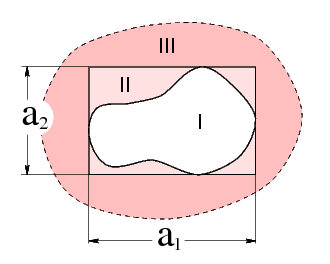
\includegraphics[scale=0.45]{img/bill_cuantico_general}
\caption{(I) Billar 2D genérico. (II) Región rectangular que encierra billar (I). (III) Región de potencial infinito.}
\label{fig:regionesbillar}
\end{figure}

La región II es una región rectangular que encierra la región I, que es la que describe las fronteras del billar que se desea estudiar.

Se parte de la ecuación de Schrödinger independiente del tiempo
\begin{equation} \label{eq:sch2d}
	\hat{H} \psi_n (\vec{r}) = \left( - \frac{\hbar^2}{2 m} \nabla^2 + V(\vec{r}) \right) \psi_n (\vec{r}) = E_n \psi_n (\vec{r}).
\end{equation}
Para resolver esta ecuación en el billar se hará una aproximación en la que se utiliza una condición de frontera de Dirichlet $ \psi (\vec{r}) |_{\vec{r} \in \bar{\Gamma}} = 0$, donde $\bar{\Gamma}$ es la frontera de la región II, es decir, una frontera rectangular, y se supondrá un potencial $V_0$ muy grande, de manera que para fines computacionales sea comparable a un potencial infinito. Con esta condición de frontera las soluciones se pueden expresar en términos de
\begin{equation} \label{eq:psi}
	\psi (\vec{r}) = \sum_m c_m \phi_m (\vec{r}),
\end{equation}
donde $c_m$ son coeficientes de expansión a ser determinados, y
\[
	\phi_m (\vec{r}) \equiv \phi_{m_1,m_2} (x_1, x_2) = \sqrt{\frac{2}{a_1}} \hbox{sen} \left( \frac{\pi}{a_1} m_1 x_1 \right) \sqrt{\frac{2}{a_2}} \hbox{sen} \left( \frac{\pi}{a_2} m_2 x_2 \right).
\]
Estas funciones $\phi_m$ forman un conjunto ortonormal, de manera que
\[
	\int d \vec{r} \phi_n (\vec{r}) \phi_m (\vec{r}) = \delta_{nm}.
\]
Se inserta la ecuación \ref{eq:psi} en la ecuación \ref{eq:sch2d}:
\[
	\hat{H} \sum_m c_m \phi_m (\vec{r}) = E_n \sum_m c_m \phi_m (\vec{r}),
\]

\[
	\sum_m \left( \hat{H} \phi_m (\vec{r}) - E_n \phi_m (\vec{r}) \right) c_m = 0.
\]
Se multiplica por $\phi_m (\vec{r})$ en la izquierda
\[
	\sum_m \left( \phi_n (\vec{r}) \hat{H} \phi_m (\vec{r}) - \phi_n(\vec{r}) E_n \phi_m (\vec{r}) \right) c_m = 0,
\]
y al integrar en todo el espacio respecto al vector de posición se obtiene
\[
	\sum_m \left( \int d \vec{r} \left[ \phi_n (\vec{r}) \hat{H} \phi_m (\vec{r}) \right] - E_n \int d \vec{r} \left[ \phi_n(\vec{r}) \phi_m (\vec{r}) \right] \right) c_m = 0,
\]
\begin{equation} \label{eq:eigen}
	\sum_m \left( H_{nm} - E_n \delta_{nm} \right) c_m = 0,
\end{equation}
que es la ecuación de eigenvalores que se desea resolver.
Para esto es necesario encontrar la forma del hamiltoniano $H_{nm}$. Partiendo de
\[
	\hat{H} = - \frac{\hbar^2}{2 m} \left( \frac{\partial^2}{\partial x_1^2} + \frac{\partial^2}{\partial x_2^2} \right) + V(\vec{r}),
\]
se obtiene
\begin{align*}
	H_{nm} &= \int d^2 \vec{r} \phi_n (\vec{r}) \hat{H} \phi_m (\vec{r}) \\
	&= \int  d^2 \vec{r} \left[ \frac{\hbar^2 \pi^2}{2 m} \left( \frac{m_1^2}{a_1^2} + \frac{m_2^2}{a_2^2} \right) \phi_n (\vec{r}) \phi_m (\vec{r}) + V(\vec{r}) \phi_n (\vec{r}) \phi_m (\vec{r}) \right].
\end{align*}
Por la forma del potencial es necesario definir
\begin{equation}
	\nu_{nm} = \int_{II} d^2 \vec{r} \phi_n (\vec{r}) \phi_m (\vec{r}),
\end{equation}
quedando así
\begin{align*}
	H_{nm} &= \int_{II}  d^2 \vec{r} \left[ \frac{\hbar^2 \pi^2}{2 m} \left( \frac{m_1^2}{a_1^2} + \frac{m_2^2}{a_2^2} \right) \phi_n (\vec{r}) \phi_m (\vec{r}) + V_0 \phi_n (\vec{r}) \phi_m (\vec{r}) \right] \\
	&= \frac{\hbar^2 \pi^2}{2 m} \left( \frac{m_1^2}{a_1^2} + \frac{m_2^2}{a_2^2} \right) \delta_{nm} + V_0 \nu_{nm}.
\end{align*}

De esta manera se puede resolver la ecuación \ref{eq:eigen}, y al obtener sus eigenvalores y eigenfunciones se conocen sus niveles de energía y soluciones respectivamente.

Con esto se puede implementar un método numérico para encontrar las soluciones. Debido a los límites computacionales es necesario restringir el número de términos $M$ en la expansión descrita en la ecuación \ref{eq:psi}, ya que el tamaño de la matriz $H_{nm}$ que se desea calcular será de $M^2 \times M^2$.
Los pasos para resolver el sistema son:

\begin{enumerate}
\item Escoger los valores $M$ y $V_0$ considerando la precisión del software/hardware y la duración de cómputo deseada.
\item Definir las fronteras del sistema.
\item Calcular todos los elementos  de $\nu_{nm}$ numérica o analíticamente utilizando la frontera definida.
\item Construir $H_{nm}$.
\item Obtener eigenvalores y eigenvectores de $H_{nm}$, que corresponden a $E_n$ y $c_m$.
\end{enumerate}

\renewcommand*{\refname}{}
\begin{thebibliography}{100}

\bibitem{EM} David L. Kaufman, et al. Expansion method for stationary states of quantum billiards. Am. J. Phys., Vol. 67, No. 2, February 1999.

\end{thebibliography}

\end{document}

